\documentclass[a4paper,11pt,oneside]{report}

\usepackage[UKenglish]{babel}

\usepackage{xcolor}
\usepackage{graphicx}

\usepackage{caption}

\title{3F --- Framework for \textsc{Femm}}
\author{}

\begin{document}
\maketitle
\tableofcontents

\chapter{Geometry}

\section{Slots}
\makebox[1\textwidth][c]{
\begin{tabular}{ccccccc}
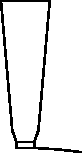
\includegraphics{../examples/slots/squared_slot} &
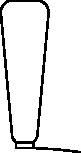
\includegraphics{../examples/slots/rounded_slot} &
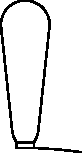
\includegraphics{../examples/slots/round_slot} &
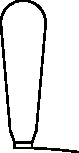
\includegraphics{../examples/slots/semiround_slot} &
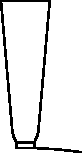
\includegraphics{../examples/slots/roundsemi_slot} &
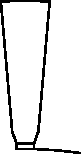
\includegraphics{../examples/slots/semiarc_slot} &
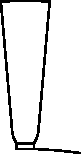
\includegraphics{../examples/slots/roundarc_slot} \\
%
\texttt{squared} &
\texttt{rounded} &
\texttt{round} &
\texttt{semiround} &
\texttt{roundsemi} &
\texttt{semiarc} & 
\texttt{roundarc}
\end{tabular}}
\vspace{1cm}


% Stators
\newpage
\section{Stators}
\begin{tabular}{c}
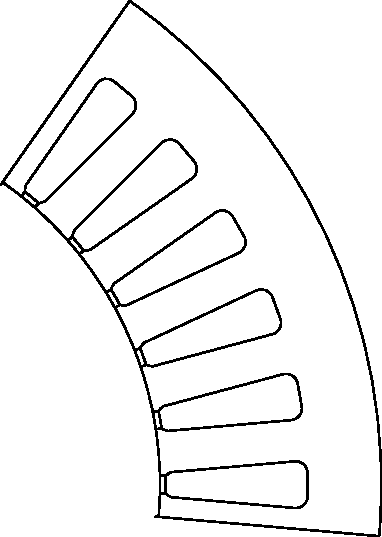
\includegraphics[scale=0.75]{../examples/stators/1pole} 
\\
$ 1 $ \texttt{pole}
\end{tabular}
\vspace{5mm}

\begin{tabular}{c}
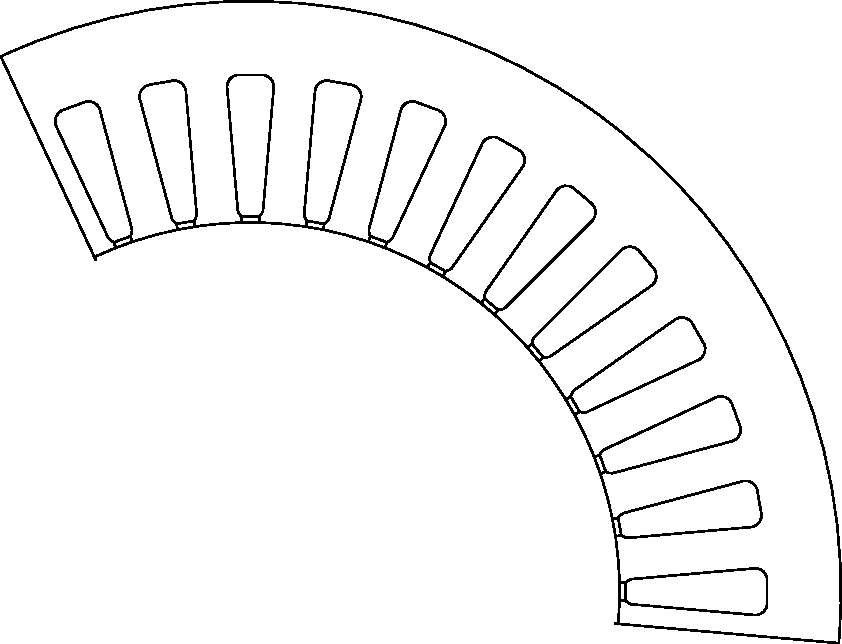
\includegraphics[scale=0.75]{../examples/stators/2pole} 
\\
$ 2 $ \texttt{poles}
\end{tabular}
\vspace{5mm}

\begin{tabular}{c}
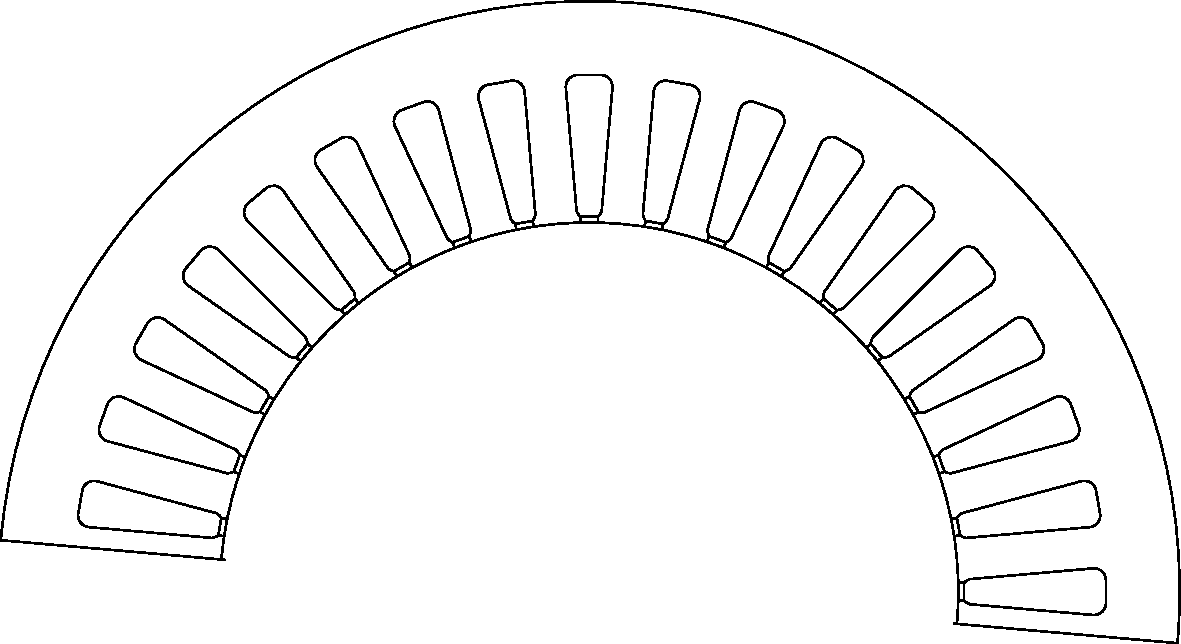
\includegraphics[scale=0.75]{../examples/stators/ppole} 
\\
$ p $ \texttt{poles}
\end{tabular}
\vspace{5mm}

\begin{tabular}{c}
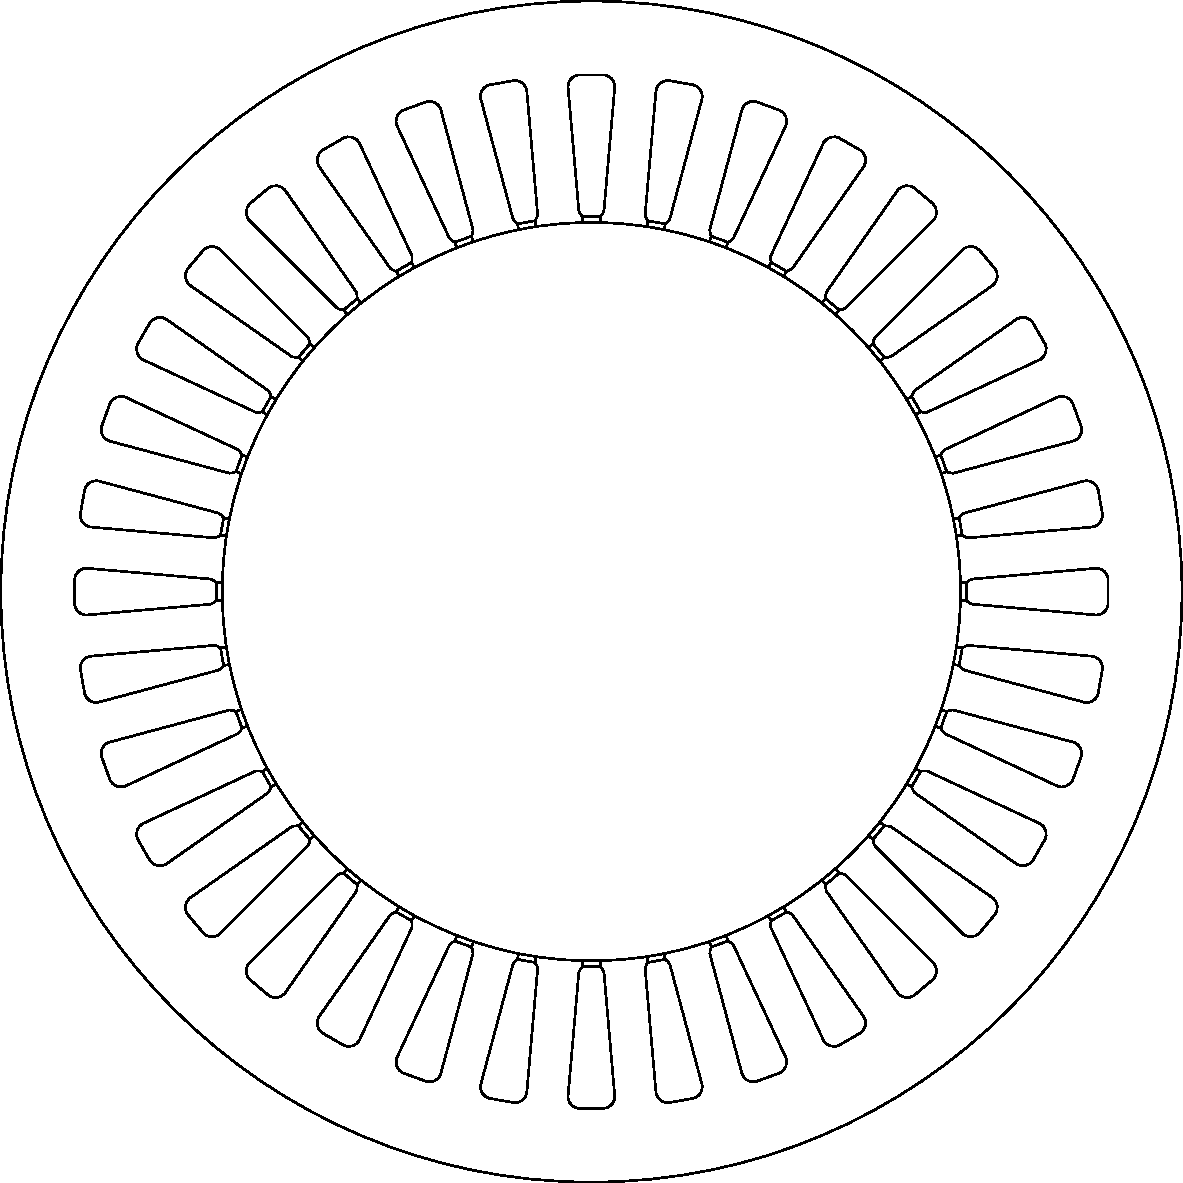
\includegraphics[scale=0.75]{../examples/stators/2ppole}
 
\\
$ 2p $ \texttt{poles}
\end{tabular}



% Magnets
\newpage
\section{SPM Magnets}

\begin{tabular}{c}
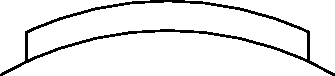
\includegraphics[scale=1]{../examples/magnets/parallel_rect}
\\
\texttt{parallel + rect}
\end{tabular}
\vspace{5mm}

\noindent
\begin{tabular}{c}
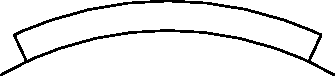
\includegraphics[scale=1]{../examples/magnets/parallel_trapz}
\\
\texttt{parallel + trapz}
\end{tabular}
\vspace{5mm}

\noindent
\begin{tabular}{c}

\includegraphics[scale=1]{../examples/magnets/radial_trapz}
\\
\texttt{radial (+ trapz)}
\end{tabular}




% Rotors
\newpage
\section{SPM Rotors}
\begin{tabular}{c}
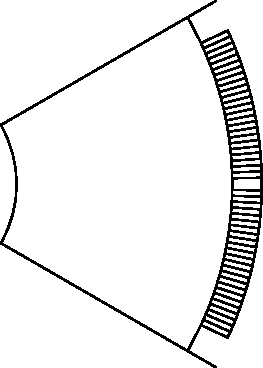
\includegraphics[scale=0.75]{../examples/rotors/1pole} 
\\
$ 1 $ \texttt{pole}
\end{tabular}
\vspace{5mm}

\begin{tabular}{c}
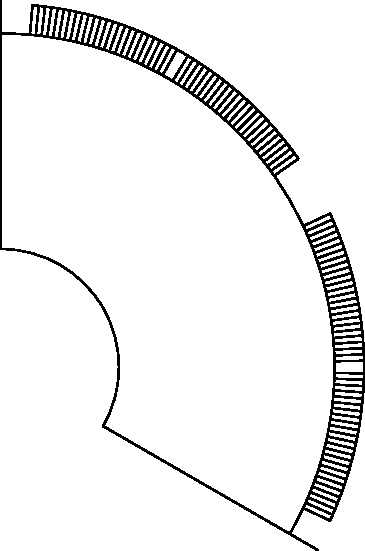
\includegraphics[scale=0.75]{../examples/rotors/2pole} 
\\
$ 2 $ \texttt{poles}
\end{tabular}
\vspace{5mm}

\begin{tabular}{c}
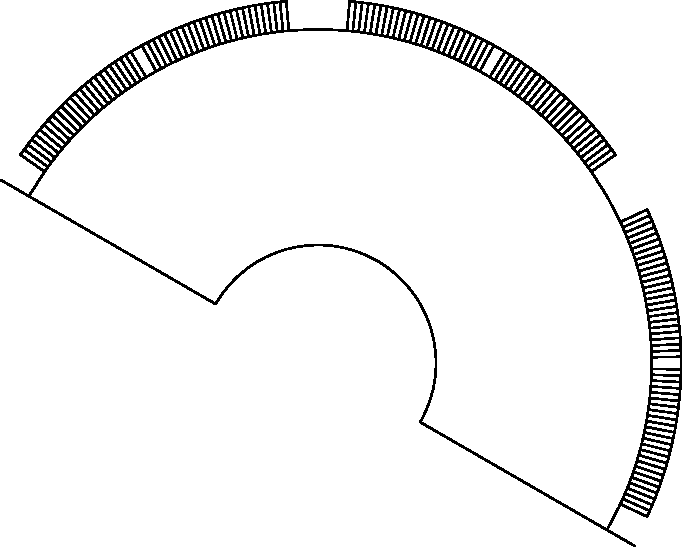
\includegraphics[scale=0.75]{../examples/rotors/ppole} 
\\
$ p $ \texttt{poles}
\end{tabular}
\vspace{5mm}

\begin{tabular}{c}
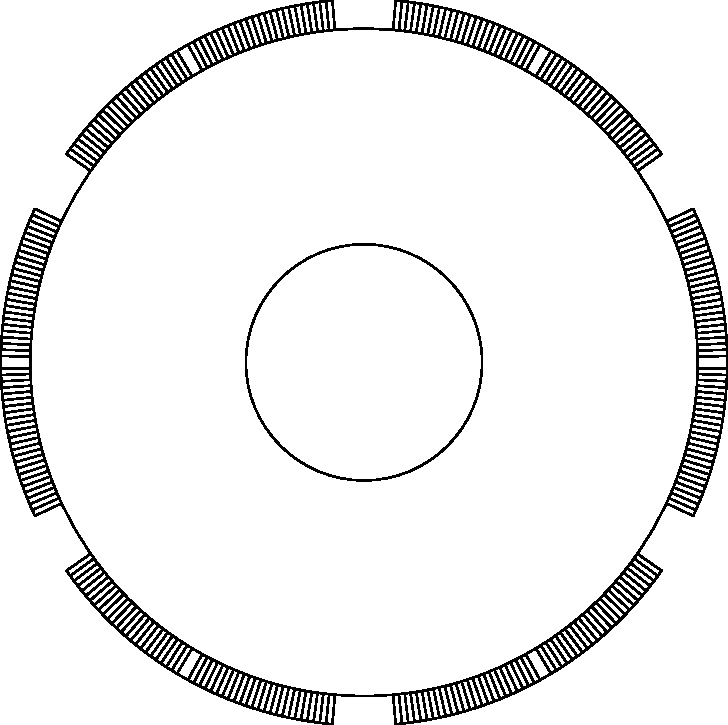
\includegraphics[scale=0.75]{../examples/rotors/2ppole} 
\\
$ 2p $ \texttt{poles}
\end{tabular}




\chapter{Winding}



\end{document}